% =================================================================================================
% File:			server_tier/miner.tex
% Description:	Definisce la sezione relativa al back-end dell'applicazione
% Created:		2015-04-07
% Author:		Cusinato Giacomo
% Email:		cusinato.giacomo@mashup-unipd.it
% =================================================================================================
% Modification History:
% Version		Modifier Date		Change											Author
% 0.0.1
% =================================================================================================

% CONTENUTO DEL CAPITOLO


\subsubsection{server::miner} % (fold)
\label{ssub:bdsm_app_server_miner}
\begin{figure}[htbp]
	\centering
	\centerline{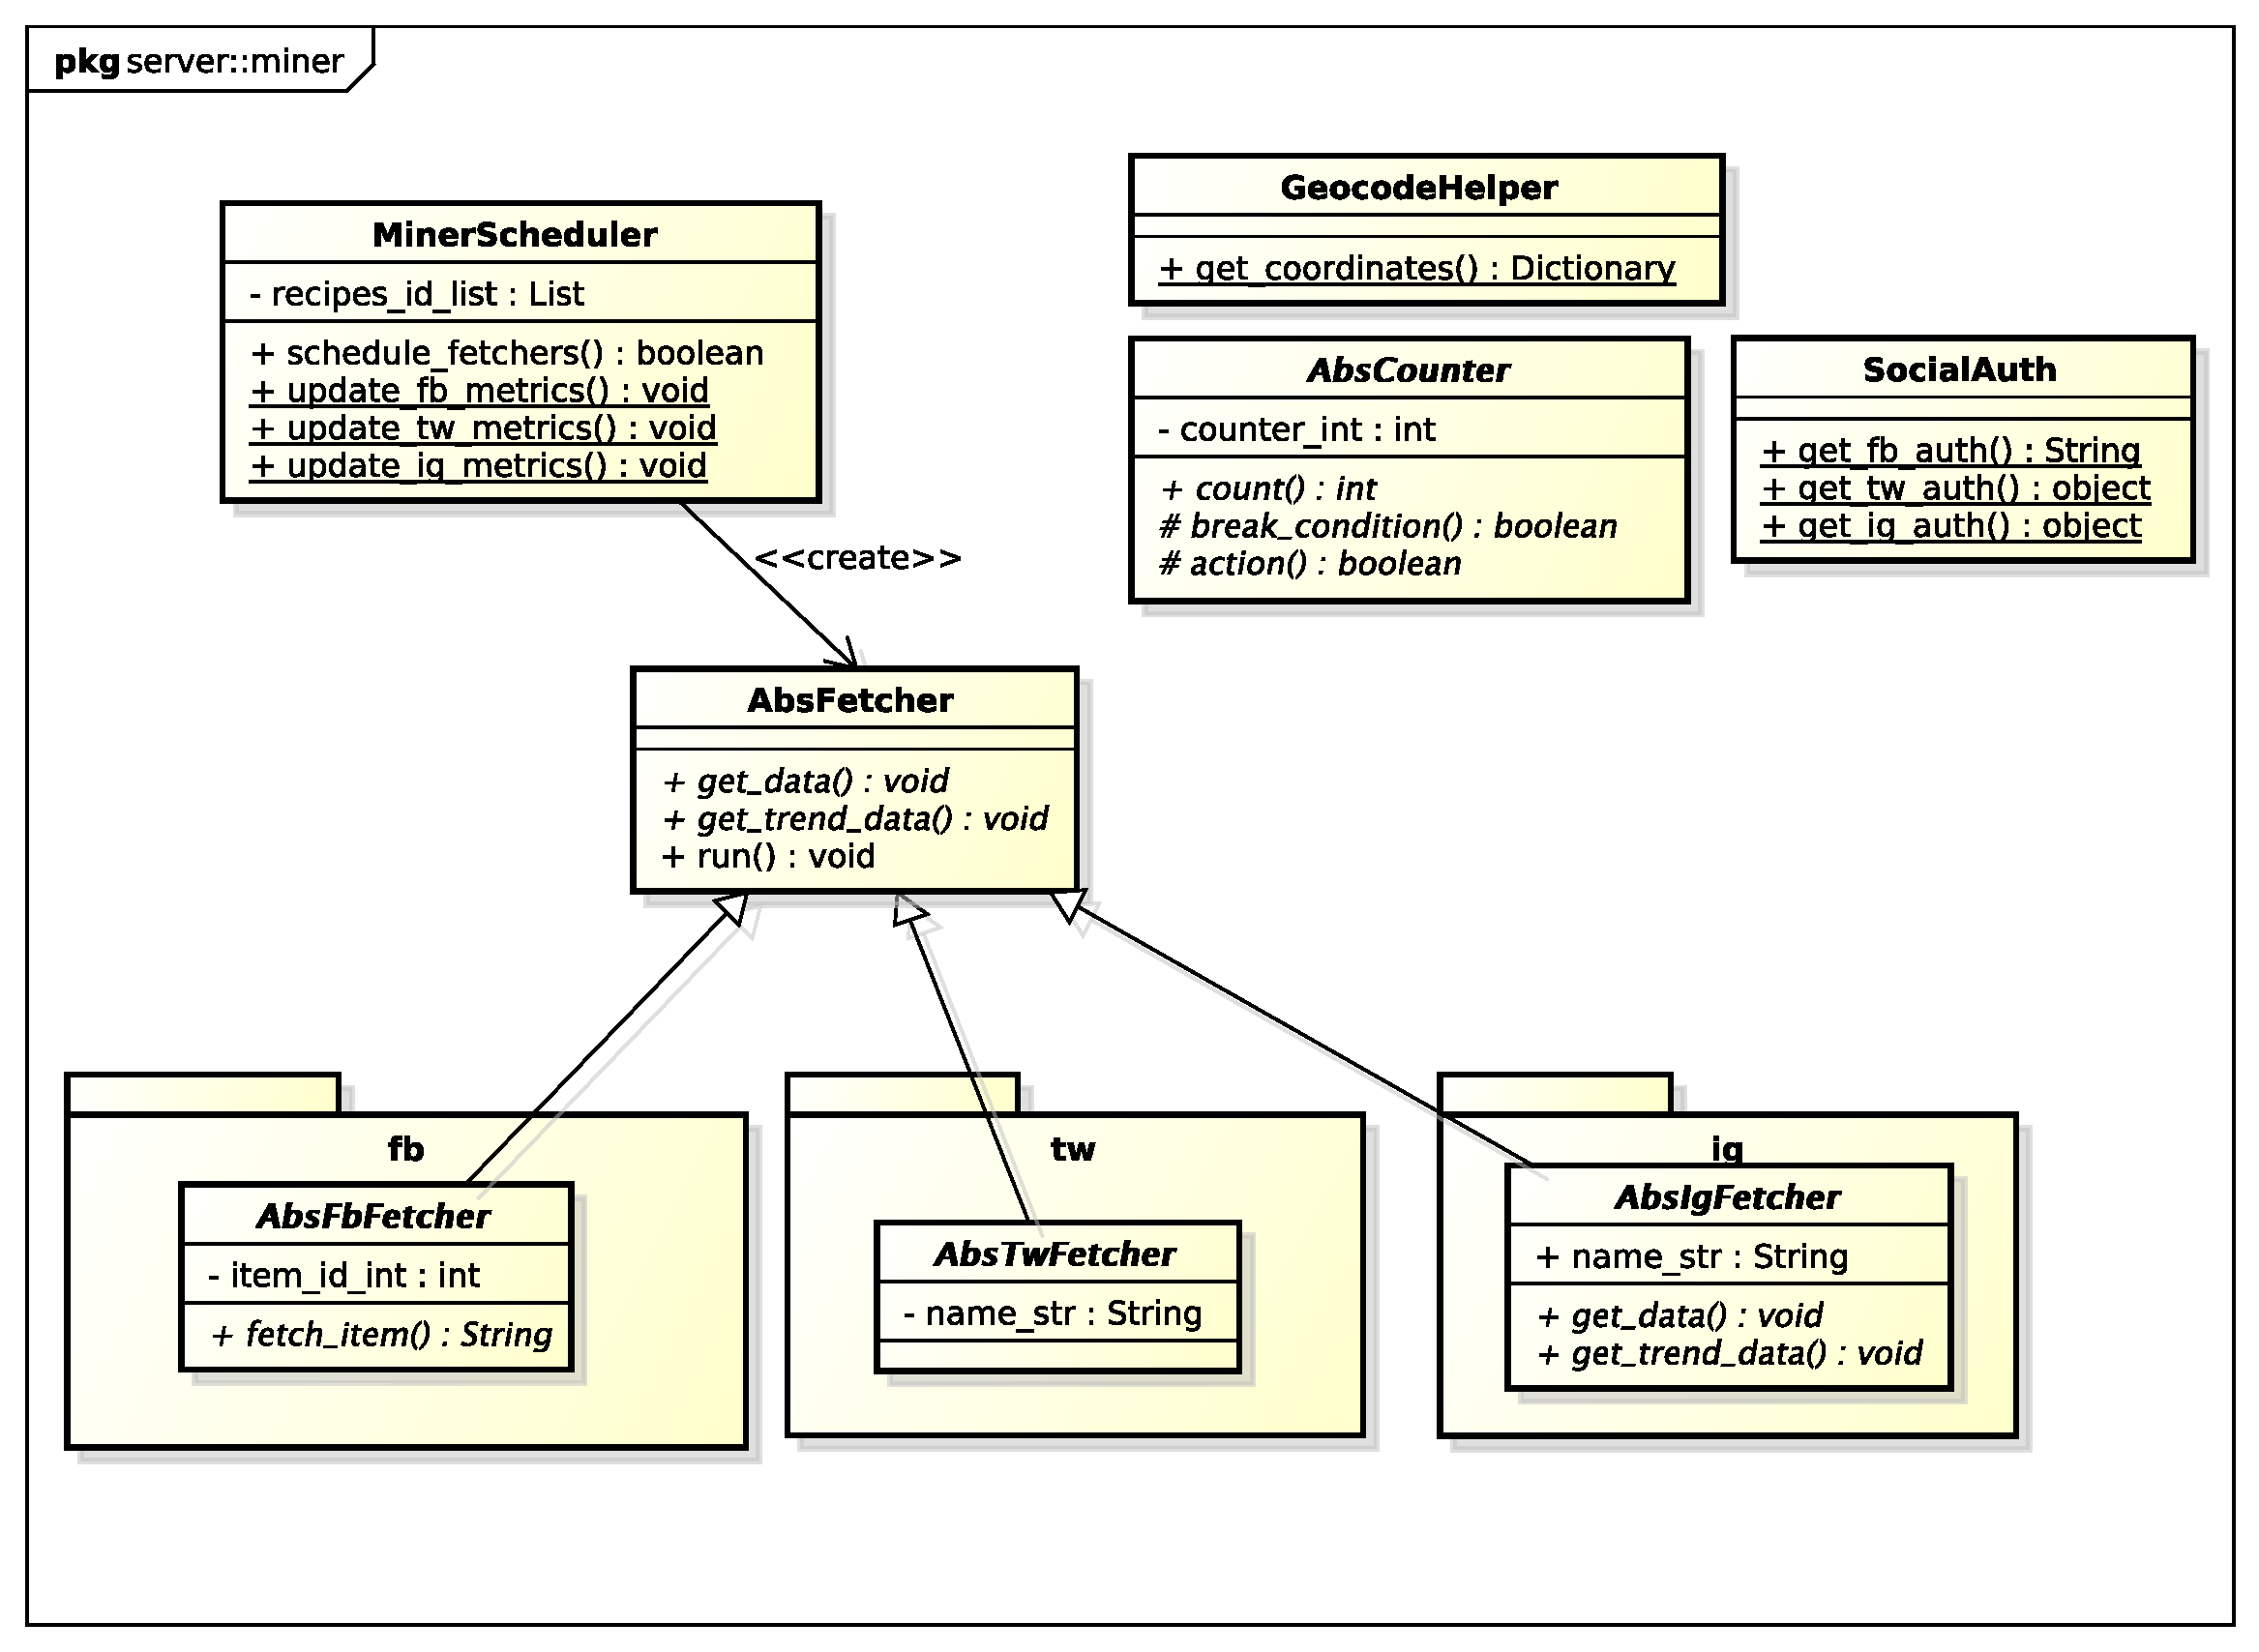
\includegraphics[scale=0.4]{./images/server/miner.pdf}}
	\caption{Package - server::miner}
\end{figure}

\begin{itemize}
  \item \textbf{Descrizione}: è il package che contiene tutte le classi che includono i metodi per prelevare i dati grezzi dai vari social network e salvarli nel database;
  \item \textbf{Padre}: server
  \item \textbf{Package contenuti}:
  	\begin{itemize}
  		\item server::miner::fb
  		\item server::miner::ig
  		\item server::miner::tw
  	\end{itemize}
  \item \textbf{Interazione con altri componenti}:
  	\begin{itemize}
  		\item server::processor
  		\item server::db
  	\end{itemize}
\end{itemize}

\paragraph{Classi} % (fold)
		\subparagraph{server::miner::MinerScheduler} % (fold)
		\label{subp:server_miner_MinerScheduler}
			\begin{itemize}
				\item \textbf{Descrizione}: classe che si occupa di creare i fetcher che preleveranno i dati per ogni metrica di ogni social network;
				\item \textbf{Utilizzo}: contiene la lista degli id delle Recipe da aggiornare ed un metodo che inizializza e avvia i vari fetcher;
				\item \textbf{Relazioni con altre classi}:
					\begin{itemize}
						\item server::miner::AbsFetcher
					\end{itemize}
				\item \textbf{Attributi}: TO DO
				\item \textbf{Metodi}: TO DO
			\end{itemize}
		% subparagraph server_miner_MinerScheduler [end]

		\subparagraph{server::miner::AbsCounter} % (fold)
		\label{subp:server_miner_AbsCounter}
			\begin{itemize}
				\item \textbf{Descrizione}: classe astratta che rappresenta il padre delle classi counter delle varie metriche;
				\item \textbf{Utilizzo}: descrive lo scheletro dell'algoritmo di counting necessario ad effettuare il conteggio di determinati dati ricavati con lo scopo ottenere un trend;
				\item \textbf{Relazioni con altre classi}:
					\begin{itemize}
						\item server::miner::fb::AbsFbCounter
						\item server::miner::tw::AbsTwCounter
						\item server::miner::ig::AbsIgCounter
					\end{itemize}
				\item \textbf{Attributi}: TO DO
				\item \textbf{Metodi}: TO DO
			\end{itemize}
		% subparagraph server_miner_AbsCounter [end]

		\subparagraph{server::miner::AbsFetcher} % (fold)
		\label{subp:server_miner_AbsFetcher}
				\begin{itemize}
				\item \textbf{Descrizione}: classe astratta che rappresenta il padre delle classi fetcher dei vari social network;
				\item \textbf{Utilizzo}: è utilizzata per mantenere l'estensibilità nel caso l'applicazione venga estesa con altre API  oltre a quelli dei social network presi in considerazione;
				\item \textbf{Relazioni con altre classi}:
					\begin{itemize}
						\item server::miner::fb::AbsFbFetcher
						\item server::miner::tw::AbsTwFetcher
						\item server::miner::ig::AbsIgFetcher
					\end{itemize}
				\item \textbf{Attributi}: TO DO
				\item \textbf{Metodi}: TO DO
			\end{itemize}
		% subparagraph server_miner_AbsFetcher [end]

\subsubsection{server::miner::fb} % (fold)
\label{ssub:bdsm_app_server_miner_fb}
\begin{figure}[htbp]
	\centering
	\centerline{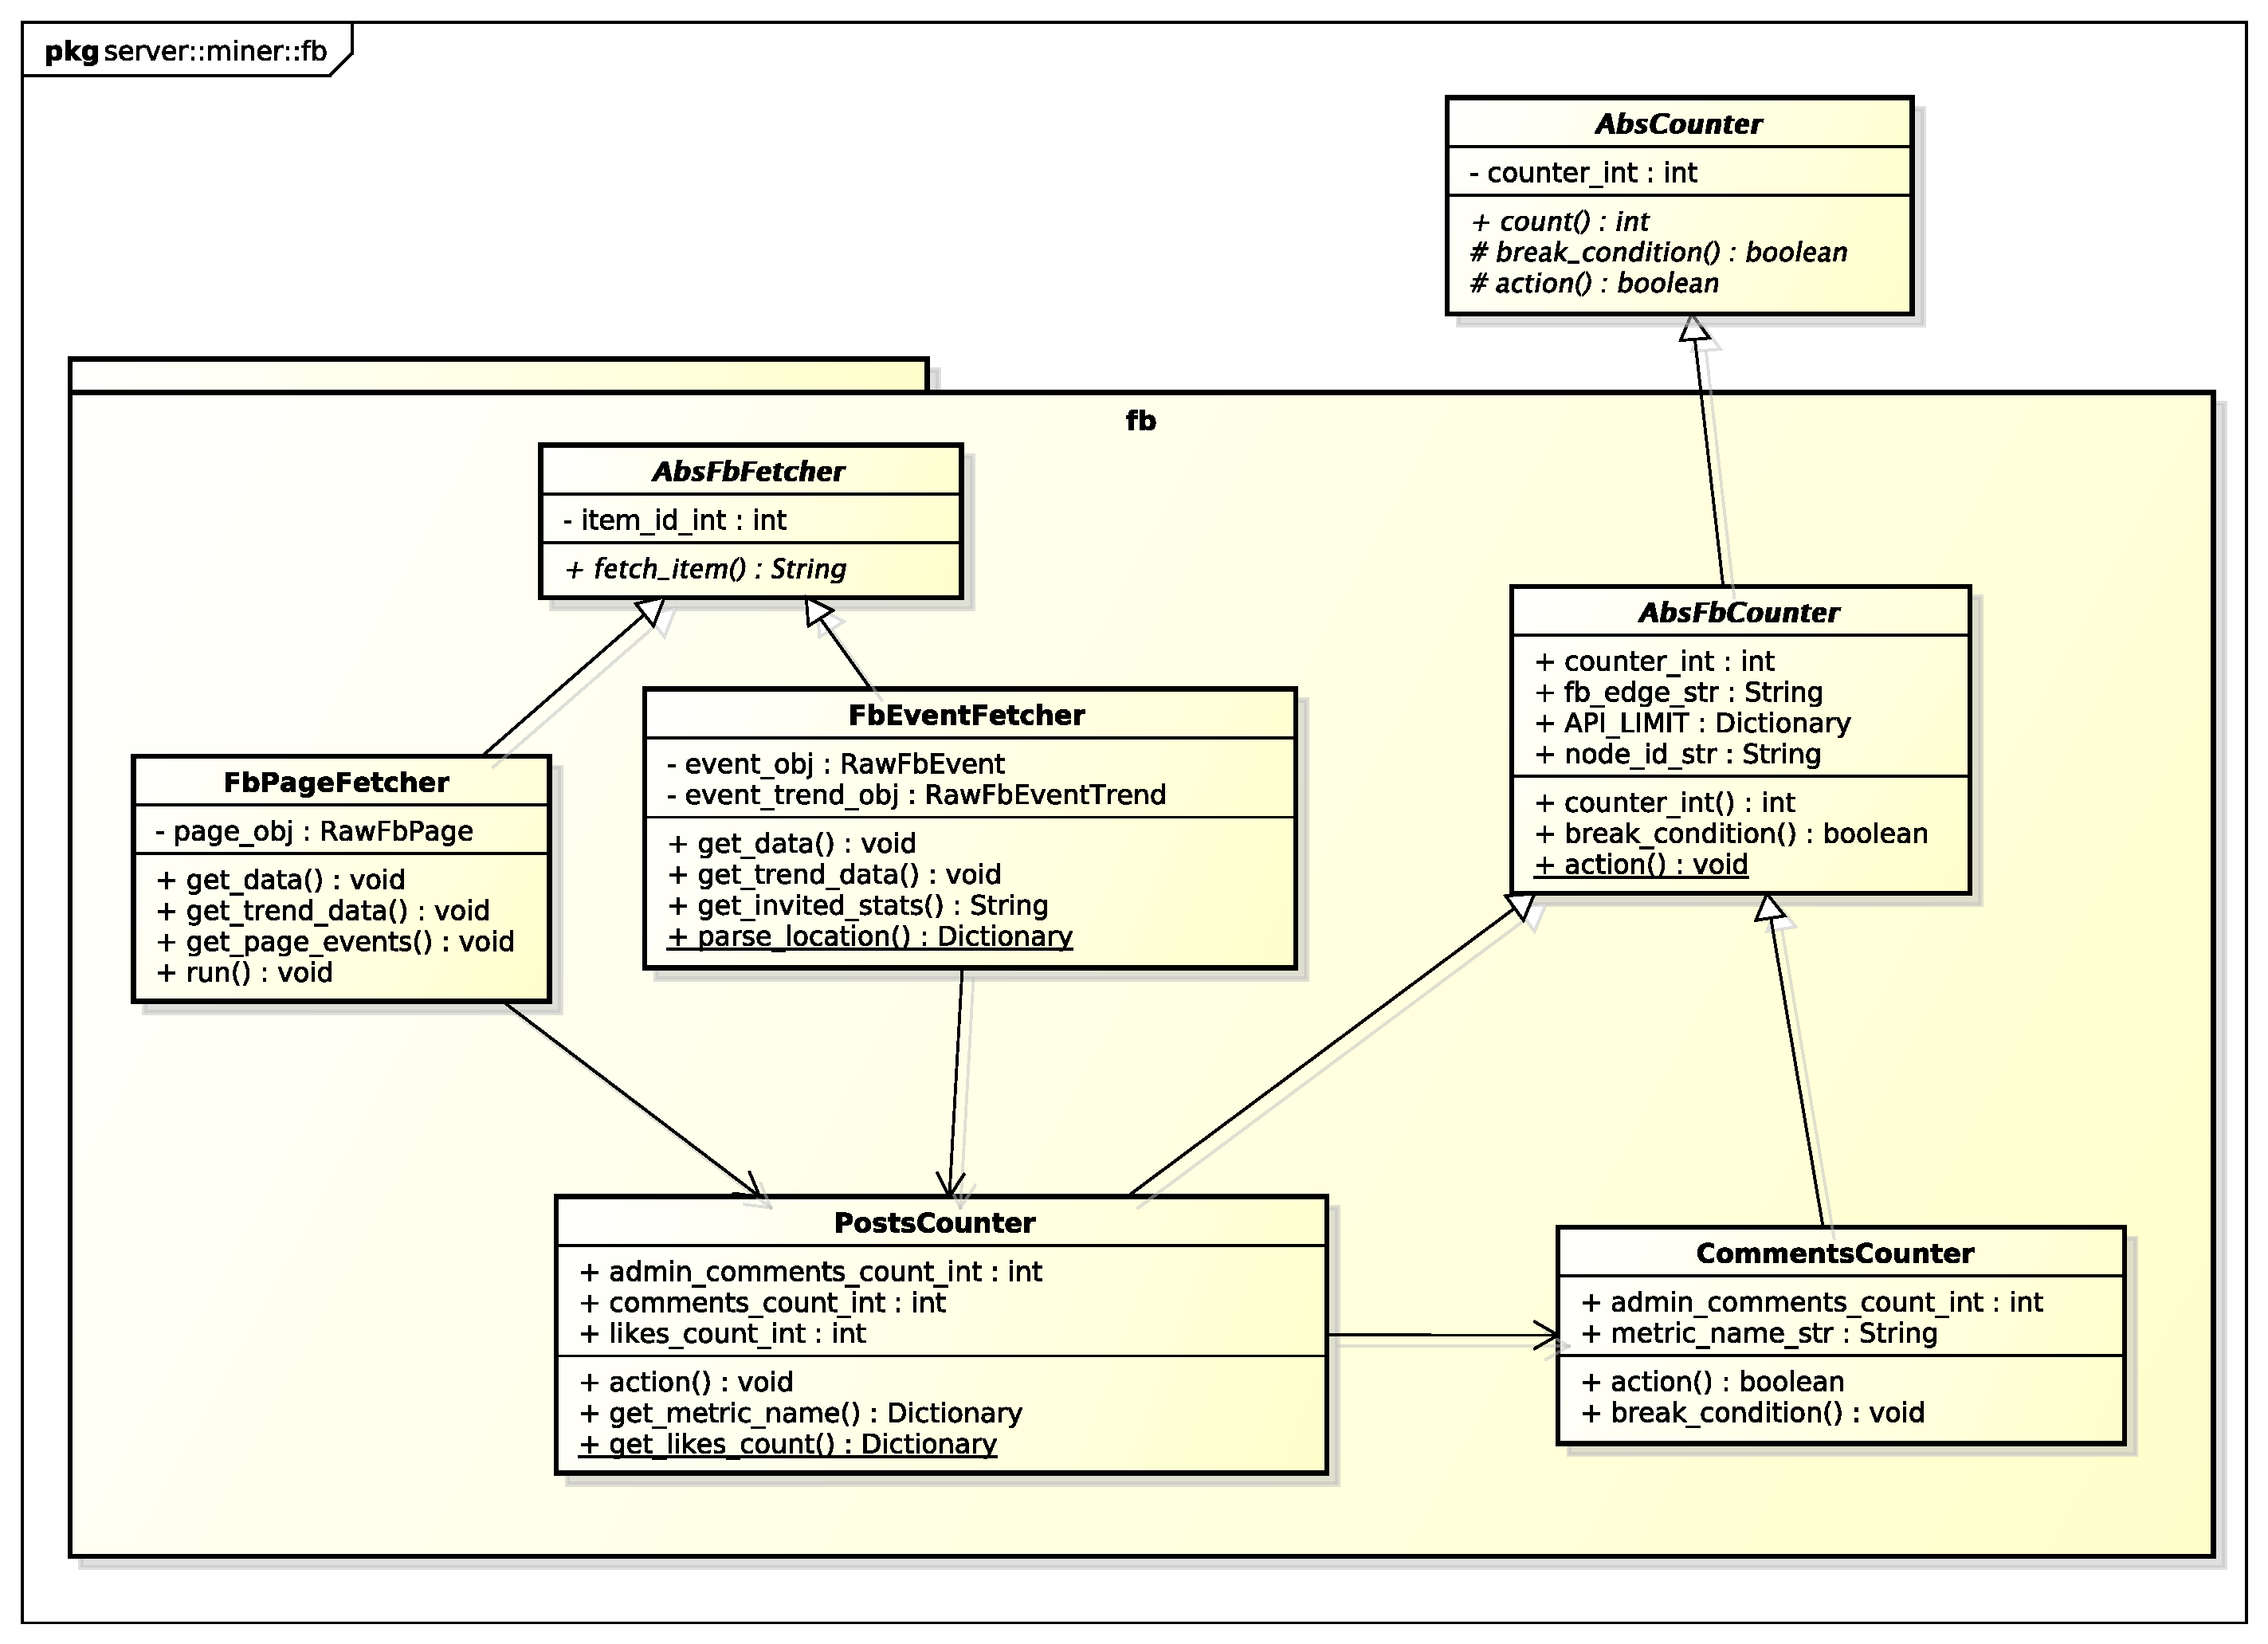
\includegraphics[scale=0.3]{./images/server/miner_fb.pdf}}
	\caption{Package - server::miner::fb}
\end{figure}

\begin{itemize}
  \item \textbf{Descrizione}: è il package che contiene tutte le classi che includono i metodi per prelevare i dati da Facebook e salvarli nel database;
  \item \textbf{Padre}: server::miner
  \item \textbf{Interazione con altri componenti}:
  	\begin{itemize}
  		\item server::db
  	\end{itemize}
\end{itemize}

	\paragraph{Classi} % (fold)
		\subparagraph{server::miner::fb::AbsFbFetcher} % (fold)
		\label{subp:server_miner_fb_AbsFbFetcher}
			\begin{itemize}
				\item \textbf{Descrizione}: classe astratta che rappresenta il padre di ogni fetcher relativo a Facebook;
				\item \textbf{Utilizzo}: contiene un metodo che ricava i dati statici di un'entità Facebook ed un metodo astratto che verrà definito nelle classi figlie;
				\item \textbf{Classi ereditate}: server::miner::AbsFetcher
				\item \textbf{Relazioni con altre classi}:
					\begin{itemize}
						\item server::miner::fb::FbPageFetcher
						\item server::miner::fb::FbEventFetcher
					\end{itemize}
				\item \textbf{Attributi}: TO DO
				\item \textbf{Metodi}: TO DO
			\end{itemize}
	% subparagraph server_miner_fb_AbsFbFetcher [end]

		\subparagraph{server::miner::fb::FbPageFetcher} % (fold)
		\label{subp:server_miner_fb_FbPageFetcher}
			\begin{itemize}
				\item \textbf{Descrizione}: classe che si occupa ricava i dati dalle pagine Facebook;
				\item \textbf{Utilizzo}: contiene un campo che descrive i dati statici di una pagina, un campo che descrive i dati dinamici ed un metodo che li ricava tramite l'utilizzo della classe \texttt{PostCounter};
				\item \textbf{Classi ereditate}: server::miner::fb::AbsFbFetcher
				\item \textbf{Relazioni con altre classi}:
					\begin{itemize}
						\item server::miner::fb::PostCounter
					\end{itemize}
				\item \textbf{Attributi}: TO DO
				\item \textbf{Metodi}: TO DO
			\end{itemize}
		% subparagraph server_miner_fb_FbPageFetcher [end]

		\subparagraph{server::miner::fb::FbEventFetcher} % (fold)
		\label{subp:server_miner_fb_FbEventFetcher}
			\begin{itemize}
				\item \textbf{Descrizione}: classe che ricava i dati di un evento Facebook;
				\item \textbf{Utilizzo}: contiene un campo che descrive i dati statici di un evento, un campo che descrive i dati dinamici e un metodo che li ricava tramite l'utilizzo della classe \texttt{PostCounter};
				\item \textbf{Classi ereditate}: server::miner::fb::AbsFbFetcher
				\item \textbf{Relazioni con altre classi}:
					\begin{itemize}
						\item server::miner::fb::PostCounter
						\item server::miner::fb::AttendingCounter
						\item server::miner::fb::MaybeCounter
						\item server::miner::fb::InvitedCounter
						\item server::miner::fb::RefusedCounter
					\end{itemize}
				\item \textbf{Attributi}: TO DO
				\item \textbf{Metodi}: TO DO
			\end{itemize}
	% subparagraph server_miner_fb_FbEventFetcher [end]

		\subparagraph{server::miner::fb::AbsFbCounter} % (fold)
		\label{subp:server_miner_fb_AbsFbCounter}
			\begin{itemize}
				\item \textbf{Descrizione}: classe astratta che rappresenta il padre per tutte le classi counter delle metriche di Facebook;
				\item \textbf{Utilizzo}: classe che contiene l'id delle metriche su cui effettuare il counting, questa classe effettua l'overloading dei metodi della classe padre specificando la struttura dell'algoritmo per il counting su dati Facebook;
				\item \textbf{Classi ereditate}: server::miner::AbsCounter
				\item \textbf{Relazioni con altre classi}:
					\begin{itemize}
						\item server::miner::fb::AttendingCounter
						\item server::miner::fb::MaybeCounter
						\item server::miner::fb::InvitedCounter
						\item server::miner::fb::RefusedCounter
						\item server::miner::fb::PostCounter
						\item server::miner::fb::CommentCounter
						\item server::miner::fb::LikeCounter
					\end{itemize}
				\item \textbf{Attributi}: TO DO
				\item \textbf{Metodi}: TO DO
			\end{itemize}
	% subparagraph server_miner_fb_AbsFbCounter [end]

		\subparagraph{server::miner::fb::AttendingCounter} % (fold)
		\label{subp:server_miner_fb_AttendingCounter}
			\begin{itemize}
				\item \textbf{Descrizione}: classe che descrive l'algoritmo per il counting degli invitati che non hanno ancora risposto in un evento Facebook;
				\item \textbf{Utilizzo}: classe che ricava il numero di persone invitate che non hanno ancora risposto di un evento Facebook;
				\item \textbf{Classi ereditate}: server::miner::fb::AbsFbCounter
				\item \textbf{Attributi}: TO DO
				\item \textbf{Metodi}: TO DO
			\end{itemize}
	% subparagraph server_miner_fb_AttendingCounter

		\subparagraph{server::miner::fb::MaybeCounter} % (fold)
		\label{subp:server_miner_fb_MaybeCounter}
			\begin{itemize}
				\item \textbf{Descrizione}: classe che descrive l'algoritmo per il counting dei maybe in un evento Facebook;
				\item \textbf{Utilizzo}: classe che ricava il numero di persone in forse per un evento Facebook;
				\item \textbf{Classi ereditate}: server::miner::fb::AbsFbCounter
				\item \textbf{Attributi}: TO DO
				\item \textbf{Metodi}: TO DO
			\end{itemize}
	% subparagraph server_miner_fb_MaybeCounter

	\subparagraph{server::miner::fb::InvitedCounter} % (fold)
		\label{subp:server_miner_fb_InvitedCunter}
			\begin{itemize}
				\item \textbf{Descrizione}: classe che descrive l'algoritmo per il counting degli invited in un evento Facebook;
				\item \textbf{Utilizzo}: classe che ricava il numero di persone invitate ad un evento Facebook;
				\item \textbf{Classi ereditate}: server::miner::fb::AbsFbCounter
				\item \textbf{Attributi}: TO DO
				\item \textbf{Metodi}: TO DO
			\end{itemize}
	% subparagraph server_miner_fb_InvitedCounter

	\subparagraph{server::miner::fb::RefusedCounter} % (fold)
		\label{subp:server_miner_fb_RefusedCounter}
			\begin{itemize}
				\item \textbf{Descrizione}: classe che descrive l'algoritmo per il counting dei refused in un evento Facebook;
				\item \textbf{Utilizzo}: classe che ricava il numero di persone che hanno rifiutato l'invito per un evento Facebook;
				\item \textbf{Classi ereditate}: server::miner::fb::AbsFbCounter
				\item \textbf{Attributi}: TO DO
				\item \textbf{Metodi}: TO DO
			\end{itemize}
	% subparagraph server_miner_fb_RefusedCounter

	\subparagraph{server::miner::fb::PostCounter} % (fold)
		\label{subp:server_miner_fb_PostCounter}
			\begin{itemize}
				\item \textbf{Descrizione}: classe che descrive l'algoritmo per calcolare il numero dei post per ogni evento o pagina;
				\item \textbf{Utilizzo}: classe che contiene un campo per il numero dei like e un campo per il numero dei talking about per ogni post di Facebook;
				\item \textbf{Classe ereditate}: server::miner::fb::AbsFbCounter
				\item \textbf{Relazioni con altre classi}:
					\begin{itemize}
						\item server::miner::fb::CommentCounter
						\item server::miner::fb::LikeCounter
					\end{itemize}
				\item \textbf{Attributi}: TO DO
				\item \textbf{Metodi}: TO DO
			\end{itemize}
		% subparagraph server_miner_fb_PostCounter

	\subparagraph{server::miner::fb::CommentCounter} % (fold)
		\label{subp:server_miner_fb_CommentCounter}
			\begin{itemize}
				\item \textbf{Descrizione}: classe che descrive l'algoritmo per calcolare il numero di commenti per ogni post;
				\item \textbf{Utilizzo}: classe che ricava il numero di commenti per ogni post;
				\item \textbf{Classe ereditate}: server::miner::fb::AbsFbCounter
				\item \textbf{Attributi}: TO DO
				\item \textbf{Metodi}: TO DO
			\end{itemize}
	% subparagraph server_miner_fb_CommentCounter

	\subparagraph{server::miner::fb::LikeCounter} % (fold)
		\label{subp:server_miner_fb_LikeCounter}
			\begin{itemize}
				\item \textbf{Descrizione}: classe che descrive l'algoritmo per calcolare il numero di like per ogni post;
				\item \textbf{Utilizzo}: classe che ricava il numero di like per ogni post;
				\item \textbf{Classe ereditate}: server::miner::fb::AbsFbCounter
				\item \textbf{Attributi}: TO DO
				\item \textbf{Metodi}: TO DO
			\end{itemize}
	% subparagraph server_miner_fb_LikeCounter

\subsubsection{server::miner::tw} % (fold)
\label{ssub:bdsm_app_server_miner_tw}

\begin{itemize}
  \item \textbf{Descrizione}: è il package che contiene tutte le classi che includono i metodi per prelevare i dati da Twitter e salvarli nel database;
  \item \textbf{Padre}: server::miner
  \item \textbf{Interazione con altri componenti}:
  	\begin{itemize}
  		\item server::db
  	\end{itemize}
\end{itemize}

	\begin{figure}[!htbp]
		\centering
		\centerline{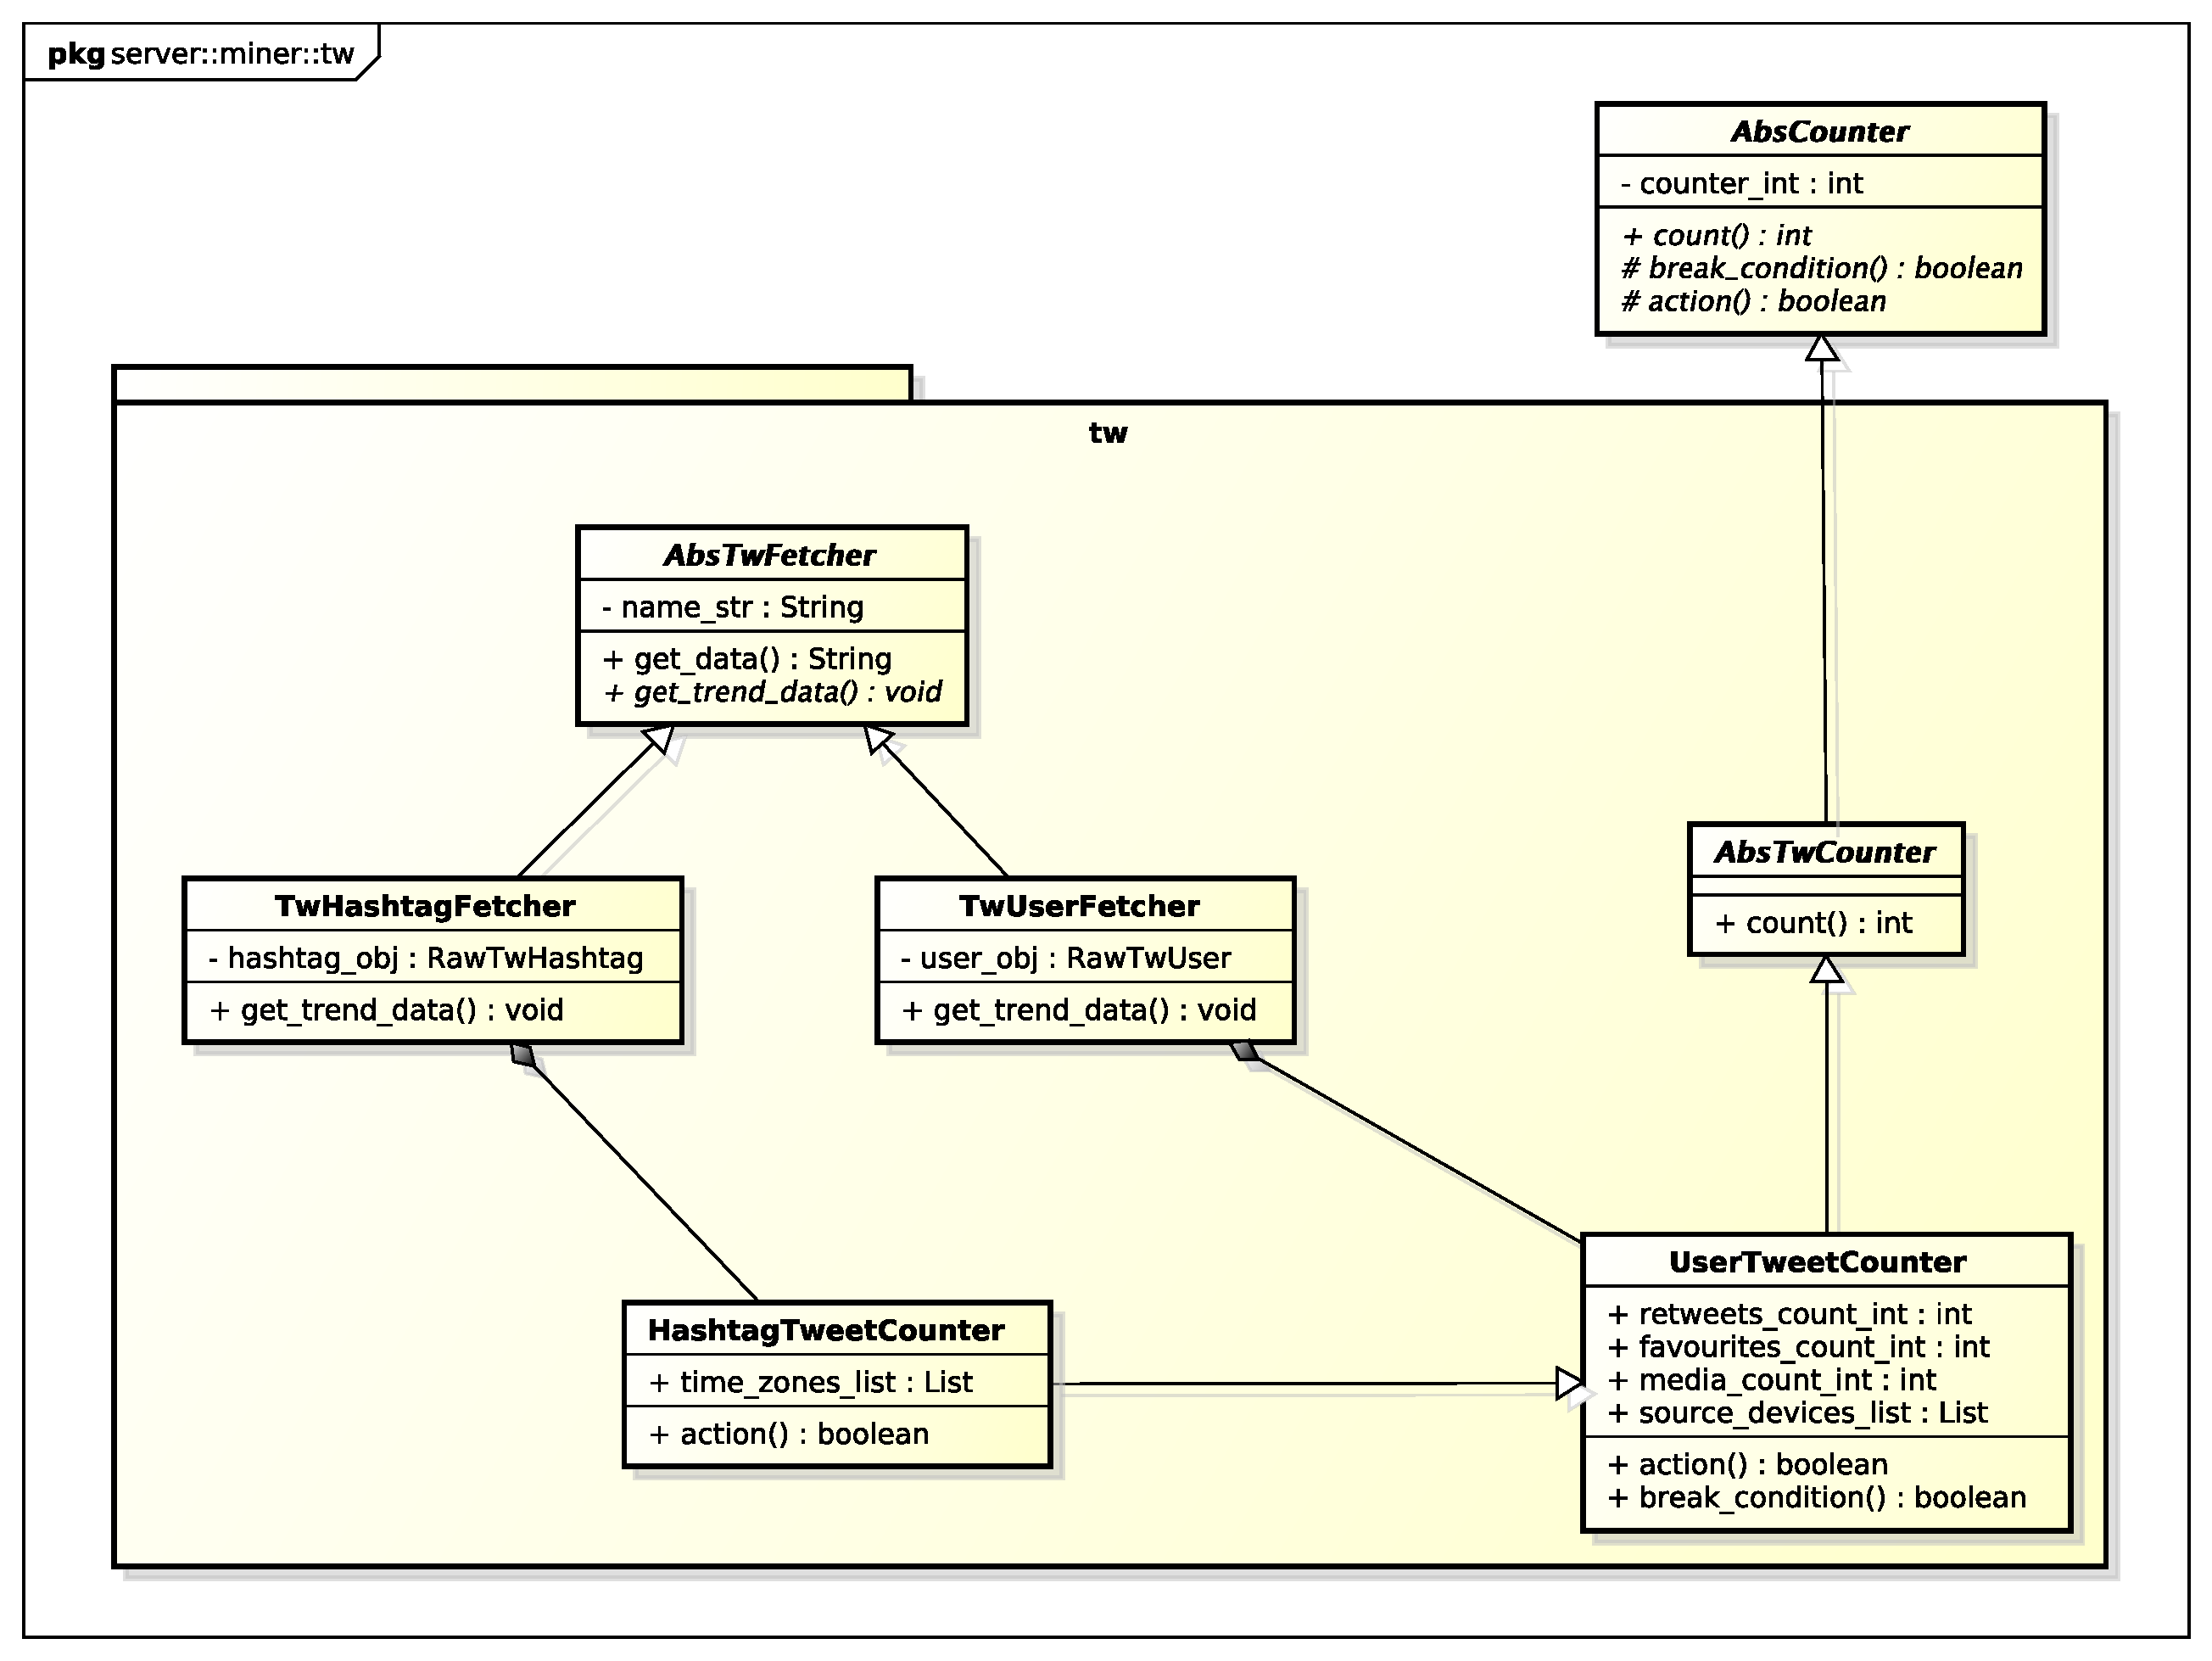
\includegraphics[scale=0.4]{./images/server/miner_tw.pdf}}
		\caption{Package - server::miner::tw}
	\end{figure}

	\paragraph{Classi} % (fold)
	\subparagraph{server::miner::tw::AbsTwFetcher} % (fold)
		\label{subp:server_miner_tw_AbsTwFetcher}
			\begin{itemize}
				\item \textbf{Descrizione}: classe astratta che rappresenta il padre di ogni fetcher relativo a Twitter;
				\item \textbf{Utilizzo}: contiene un metodo che ricava i dati statici di un'entità Twitter ed un metodo astratto che verrà definito nelle classi figlie;
				\item \textbf{Classi ereditate}: server::miner::AbsFetcher
				\item \textbf{Relazioni con altre classi}:
					\begin{itemize}
						\item server::miner::tw::TwHashtagFetcher
						\item server::miner::tw::TwUserFetcher
					\end{itemize}
				\item \textbf{Attributi}: TO DO
				\item \textbf{Metodi}: TO DO
			\end{itemize}
		% subparagraph server_miner_tw_AbsTwFetcher

	\subparagraph{server::miner::tw::TwHashtagFetcher} % (fold)
		\label{subp:server_miner_tw_TwHashtagFetcher}
			\begin{itemize}
				\item \textbf{Descrizione}: classe che ricava i dati degli hashtag di Twitter;
				\item \textbf{Utilizzo}: classe che contiene un campo che descrive i dati statici di un hashtag di Twitter e un metodo che ricava i dati dinamici tramite l'utilizzo di \texttt{HashtagTweetCounter};
				\item \textbf{Classi ereditate}: server::miner::tw::AbsTwFetcher
				\item \textbf{Relazioni con altre classi}:
					\begin{itemize}
						\item server::miner::tw::HashtagTweetCounter
					\end{itemize}
				\item \textbf{Attributi}: TO DO
				\item \textbf{Metodi}: TO DO
			\end{itemize}
		% subparagraph server_miner_tw_TwHashtagFetcher

	\subparagraph{server::miner::tw::TwUserFetcher} % (fold)
		\label{subp:server_miner_tw_TwUserFetcher}
			\begin{itemize}
				\item \textbf{Descrizione}: classe che ricava i dati degli utenti di Twitter;
				\item \textbf{Utilizzo}: classe che contiene un campo che descrive i dati statici dell'utente ed un metodo che ricava i dati dinamici tramite l'utilizzo di \texttt{UserTweetCounter};
				\item \textbf{Classi ereditate}: server::miner::tw::AbsTwFetcher
				\item \textbf{Relazioni con altre classi}:
					\begin{itemize}
						\item server::miner::tw::UserTweetCounter
					\end{itemize}
				\item \textbf{Attributi}: TO DO
				\item \textbf{Metodi}: TO DO
			\end{itemize}
		% subparagraph server_miner_tw_TwUserFetcher

	\subparagraph{server::miner::tw::AbsTwCounter} % (fold)
		\label{subp:server_miner_tw_AbsTwCounter}
			\begin{itemize}
				\item \textbf{Descrizione}: classe astratta che rappresenta il padre per tutte le classi counter delle metriche di Twitter;
				\item \textbf{Utilizzo}: oltre a contenere l’id delle metriche su cui effettuare il counting, questa classe effettua l'overloading dei metodi della classe padre specificando la struttura dell'algoritmo per il counting su dati Twitter;
				\item \textbf{Classi ereditate}: server::miner::AbsCounter
				\item \textbf{Relazioni con altre classi}:
					\begin{itemize}
						\item server::miner::UserTweetCounter
					\end{itemize}
				\item \textbf{Attributi}: TO DO
				\item \textbf{Metodi}: TO DO
			\end{itemize}
		% subparagraph server_miner_tw_AbsTwCounter

	\subparagraph{server::miner::tw::UserTweetCounter} % (fold)
		\label{subp:server_miner_tw_UserTweetCounter}
			\begin{itemize}
				\item \textbf{Descrizione}: classe che descrive l'algoritmo per il counting dei campi di un tweet, relativo ad un utente, di cui ci interessa fare un trend;
				\item \textbf{Utilizzo}: classe che ricava il numero dei retweets, il numero dei favoriti, il tipo di device, e il numero di media per ogni tweet;
				\item \textbf{Classi ereditate}: server::miner::tw::AbsTwCounter
				\item \textbf{Attributi}: TO DO
				\item \textbf{Metodi}: TO DO
			\end{itemize}
		% subparagraph server_miner_tw_UserTweetCounter


	\subparagraph{server::miner::tw::HashtagTweetCounter} % (fold)
		\label{subp:server_miner_tw_HashtagTweetCounter}
			\begin{itemize}
				\item \textbf{Descrizione}: classe che descrive l'algoritmo per il counting dei campi di un tweet, relativo ad un hashtag, di cui ci interessa fare un trend;
				\item \textbf{Utilizzo}: classe che ricava anche la time zone di ogni tweet;
				\item \textbf{Classi ereditate}: server::miner::tw::UserTweetCounter
				\item \textbf{Attributi}: TO DO
				\item \textbf{Metodi}: TO DO
			\end{itemize}
		% subparagraph server_miner_tw_HashtagTweetCounter

\subsubsection{server::miner::ig} % (fold)
\label{ssub:bdsm_app_server_miner_ig}
\begin{figure}[htbp]
	\centering
	\centerline{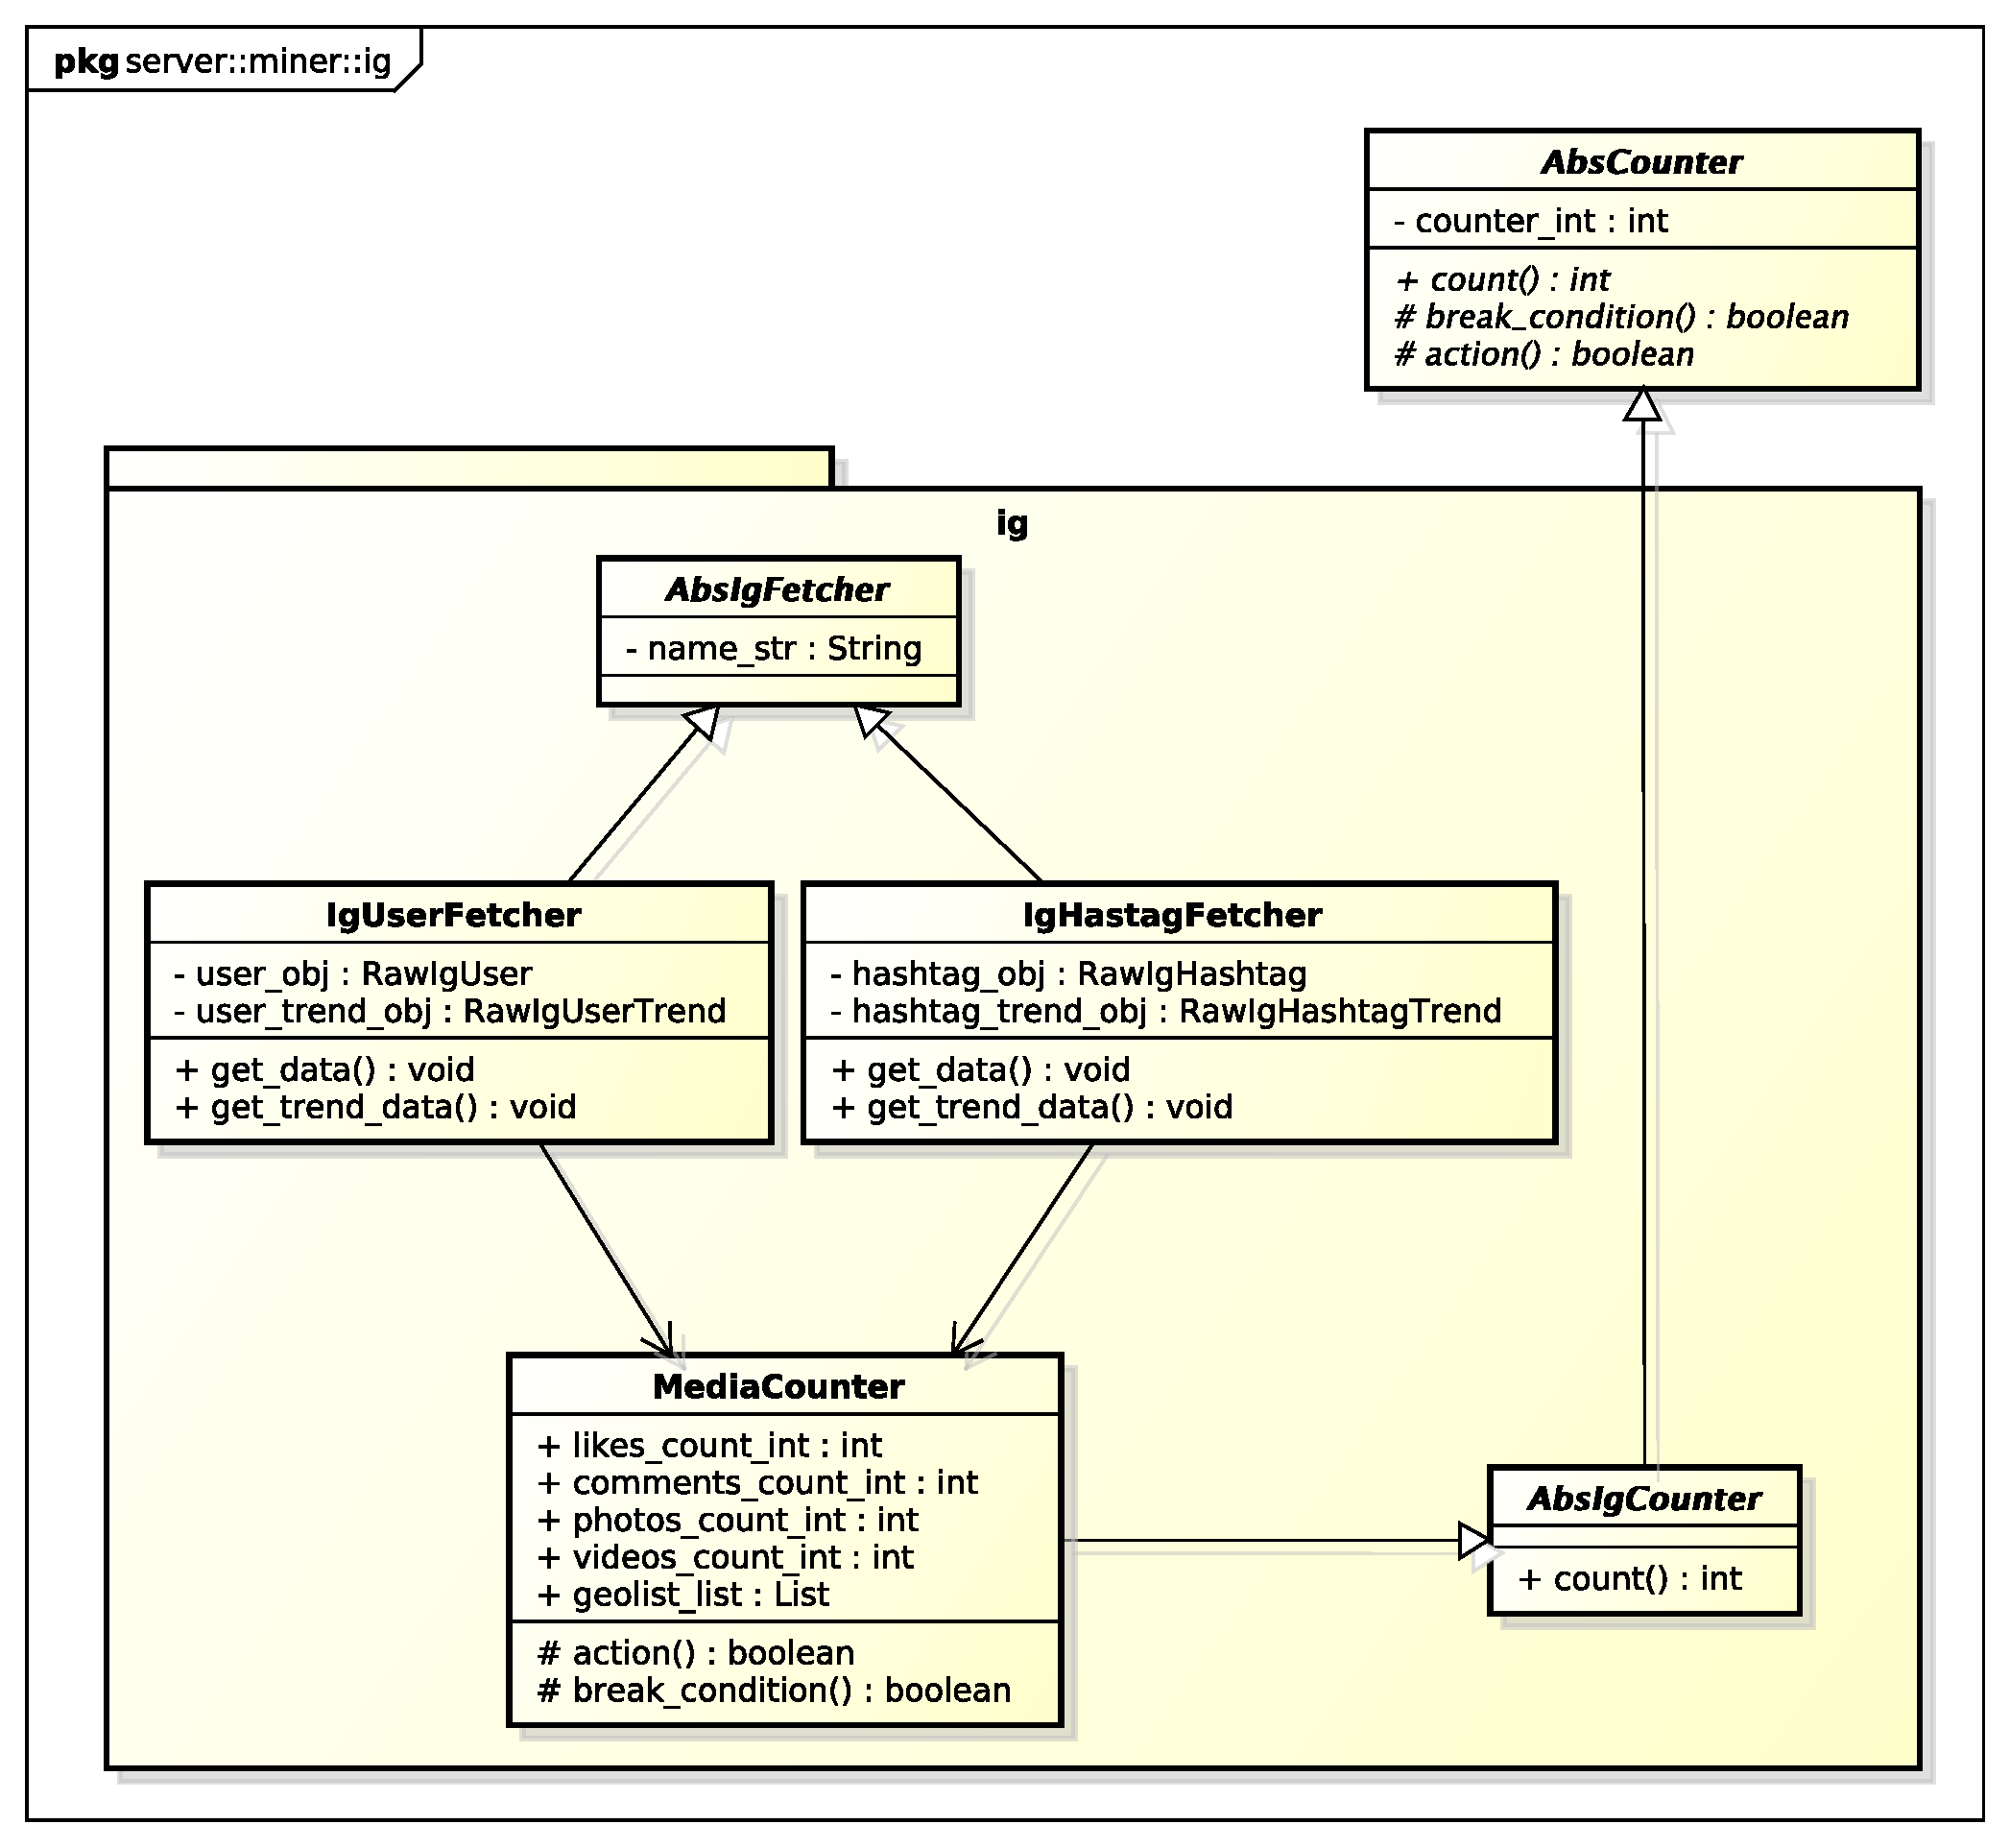
\includegraphics[scale=0.4]{./images/server/miner_ig.pdf}}
	\caption{Package - server::miner::ig}
\end{figure}


\begin{itemize}
  \item \textbf{Descrizione}: è il package che contiene tutte le classi che includono i metodi per prelevare i dati da Instagram e salvarli nel database;
  \item \textbf{Padre}: server::miner
   \item \textbf{Interazione con altri componenti}:
  	\begin{itemize}
  		\item server::db
  	\end{itemize}
\end{itemize}

	\paragraph{Classi} % (fold)
	\subparagraph{server::miner::ig::AbsIgFetcher} % (fold)
		\label{subp:server_miner_ig_AbsIgFetcher}
			\begin{itemize}
				\item \textbf{Descrizione}: classe astratta che rappresenta il padre di ogni fetcher relativo a Instagram;
				\item \textbf{Utilizzo}: contiene un metodo che ricava i dati statici di un'entità Instagram ed un metodo astratto che verrà definito nelle classi figlie;
				\item \textbf{Classi ereditate}: server::miner::AbsFetcher
				\item \textbf{Relazioni con altre classi}:
					\begin{itemize}
						\item server::miner::ig::IgUserFetcher
						\item server::miner::ig::IgHashtagFetcher
					\end{itemize}
				\item \textbf{Attributi}: TO DO
				\item \textbf{Metodi}: TO DO
			\end{itemize}
		% subparagraph server_miner_ig_AbsIgFetcher

	\subparagraph{server::miner::ig::IgUserFetcher} % (fold)
		\label{subp:server_miner_ig_IgUserFetcher}
			\begin{itemize}
				\item \textbf{Descrizione}: classe che ricava i dati dagli utenti di Instagram;
				\item \textbf{Utilizzo}: classe che contiene un campo che descrive i dati statici dell'utente ed un metodo che ricava i dati dinamici tramite l'utilizzo di \texttt{MediaCounter};
				\item \textbf{Classi ereditate}: server::miner::ig::AbsIgFetcher
				\item \textbf{Relazioni con altre classi}:
					\begin{itemize}
						\item server::miner::ig::MediaCounter
					\end{itemize}
				\item \textbf{Attributi}: TO DO
				\item \textbf{Metodi}: TO DO
			\end{itemize}
		% subparagraph server_miner_ig_IgUserFetcher

	\subparagraph{server::miner::ig::IgHashtagFetcher} % (fold)
		\label{subp:server_miner_ig_IgHashtagFetcher}
			\begin{itemize}
				\item \textbf{Descrizione}: classe che ricava i dati dagli hashtag di Instagram;
				\item \textbf{Utilizzo}: classe che contiene un campo che descrive i dati statici dell'hashtag ed un metodo che ricava i dati dinamici tramite l'utilizzo di \texttt{MediaCounter};
				\item \textbf{Classi ereditate}: server::miner::ig::AbsIgFetcher
				\item \textbf{Relazioni con altre classi}:
					\begin{itemize}
						\item server::miner::ig::MediaCounter
					\end{itemize}
				\item \textbf{Attributi}: TO DO
				\item \textbf{Metodi}: TO DO
			\end{itemize}
		% subparagraph server_miner_ig_IgHashtagFetcher

	\subparagraph{server::miner::ig::AbsIgCounter} % (fold)
		\label{subp:server_miner_ig_AbsIgCounter}
			\begin{itemize}
				\item \textbf{Descrizione}: classe astratta che rappresenta il padre per tutte le classi counter delle metriche relative ad Instagram;
				\item \textbf{Utilizzo}: classe che contiene l’id delle metriche su cui effettuare il counting, questa classe effettua l'overloading dei metodi della classe padre per specificarne l’utilizzo sui dati relativi ad Instagram;
				\item \textbf{Classi ereditate}: server::miner::AbsCounter
				\item \textbf{Relazioni con altre classi}:
					\begin{itemize}
						\item server::miner::ig::MediaCounter
					\end{itemize}
				\item \textbf{Attributi}: TO DO
				\item \textbf{Metodi}: TO DO
			\end{itemize}
		% subparagraph server_miner_ig_AbsIgCounter


	\subparagraph{server::miner::ig::MediaCounter} % (fold)
		\label{subp:server_miner_ig_MediaCounter}
			\begin{itemize}
				\item \textbf{Descrizione}: classe che descrive l'algoritmo per il counting delle metriche necessarie a descrivere il trend dei media di un utente o di un hashtag  Instagram;
				\item \textbf{Utilizzo}: classe che ricava il numero di commenti, il numero di like, il numero di foto e il numero di video di un media;
				\item \textbf{Classi ereditate}: server::miner::ig::AbsIgCounter
				\item \textbf{Attributi}: TO DO
				\item \textbf{Metodi}: TO DO
			\end{itemize}
		% subparagraph server_miner_ig_MediaCounter


% subsubsection
